\section{Results}
\label{sec:results}

Figure~\ref{fig:curve} is drawn by \texttt{figures/curve.tex} with pgfplots, so it needs no image file.
Table~\ref{tab:results} uses the booktabs rules, which the \emph{Insert a table} command also uses.

\begin{figure}[t]
  \centering
  % A plot drawn by pgfplots: no image file needed.
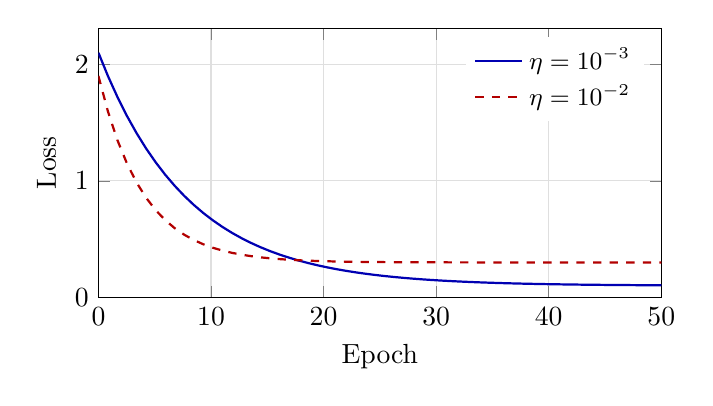
\begin{tikzpicture}
  \begin{axis}[
      width=0.72\linewidth, height=5cm,
      xlabel={Epoch}, ylabel={Loss},
      xmin=0, xmax=50, ymin=0,
      legend pos=north east, legend style={draw=none, font=\small},
      grid=major, grid style={gray!25},
    ]
    \addplot[thick, blue!70!black, domain=0:50, samples=60] {0.1 + 2*exp(-x/8)};
    \addlegendentry{$\eta = 10^{-3}$}
    \addplot[thick, red!70!black, dashed, domain=0:50, samples=60] {0.3 + 1.6*exp(-x/4)};
    \addlegendentry{$\eta = 10^{-2}$}
  \end{axis}
\end{tikzpicture}

  \caption{Training loss for two learning rates.}
  \label{fig:curve}
\end{figure}

\begin{table}[t]
  \centering
  \caption{Final loss and training time.}
  \label{tab:results}
  \begin{tabular}{lcc}
    \toprule
    Learning rate & Final loss & Time (min) \\
    \midrule
    $10^{-3}$ & 0.12 & 14 \\
    $10^{-2}$ & 0.31 & 9 \\
    \bottomrule
  \end{tabular}
\end{table}

When the paper is done, the download button above the PDF saves it, and the \emph{Changes} panel commits your work
if the folder is in git.
